\def\chapterabstract{}
\chapter{Introduction}
%\chaptermark{Introduction}
%\addcontentsline{toc}{chapter}{Introduction}

\section{Contexte}%

%Les surfaces (ou interfaces) en propagation interviennent dans de nombreuses applications scientifiques et industrielles. Elles résultent de phénomènes mettant en jeu des couplages multiphysiques complexes comme la combustion, les interactions fluide-structure, les écoulements multi-phasiques ou encore la croissance dendritique de cristaux. C’est généralement au niveau de ces surfaces qu’a lieu la physique la plus intéressante, il est donc indispensable d’en déterminer avec précision l’évolution au cours du temps\ldots
applications : simulations multi-physiques (flammes, fluide-structure, écoulements multiphasiques, multimateriaux, croissance de cristaux\ldots) CAO (usinage, planification de trajectoire de robots mobiles), infographie \ldots


\section{Formulation du problème}% d'interface en propagation}
Le problème que l'on cherche à résoudre consiste à déterminer l'évolution au cours du temps de la position d'une interface $\Gamma$ dont la vitesse instantanée de propagation $\vrm{u}$ est connue.
\subsection{Formulation lagrangienne}
%formulation lagrangienne traditionnelle (approche EDP) : vecteur vitesse 
Dans cette thèse, on se concentre sur des problèmes en trois dimensions. $\Gamma$ représente donc une surface que l'on supposera orientable et fermée.
La formulation lagrangienne traditionnelle du problème de propagation d'interface consiste à exprimer l'évolution de la position d'un point $\bx \in \Gamma$ comme une équation différentielle
\begin{equation}
	\frac{\partial \bx}{\partial t} = \vrm{u}(\bx,t).
	\label{eq:lagrange_vecteur_vitesse}
\end{equation}
La composante tangentielle du vecteur vitesse n'affecte pas la forme de l'interface. En principe, on peut donc formuler de façon équivalente la propagation de $\Gamma$ suivant un champ de vitesse normale $\nu : \Gamma \times \mathbb{R} \to \mathbb{R}$
\begin{equation}
	\frac{\partial \bx}{\partial t} = \nu(\bx,t) \unv(\bx,t),
	\label{eq:lagrange_vitesse_normale}
\end{equation}
où $\unv(\bx,t)$ désigne le vecteur normal unitaire à $\Gamma$ en $\bx$ à l'instant $t$.
Si $\vrm{u}$ et $\nu$ sont continus, et que $\Gamma$ reste régulière, la résolution des équations \eqref{eq:lagrange_vecteur_vitesse} et  \eqref{eq:lagrange_vitesse_normale} produit une solution \ldots
En revanche, lorsque $\Gamma$ présente des points singuliers où la normale n'est pas définie, cette formulation devient incomplète. 
De tels points singuliers peuvent être présents sur l'interface initiale ou bien apparaître lors de la propagation d'une interface régulière localement concave (illustration).
\begin{figure}
\centering
\definecolor{vectorcolor}{HTML}{F93802}
\definecolor{frontcolor}{HTML}{000000}
\tikzset{
  front/.style = {%
    frontcolor, %
    line width=0.8pt, %
    line join=round},%
  vector/.style = {%
    -latex', %
    line width=0.5pt, %
    vectorcolor, %
    shorten >= -2.5pt},%
  fade/.style = {%
    dash pattern=on 1.33pt off 2pt on 2pt off 2pt on 3pt off 2pt on 3.5pt off 2pt on 20pt},%
  lbl/.style = {font=\footnotesize, inner sep=2pt}}%
%
\DTLsetseparator{ }%
\DTLloaddb[noheader,keys={x,y,u,v}]{nor0}{figures/data/singularpointformation_nor_0.dat}%
%\DTLloaddb[noheader,keys={x,y,u,v}]{nor1}{figures/data/singularpointformation_nor_1.dat}%
%\DTLloaddb[noheader,keys={x,y,u,v}]{nor2}{figures/data/singularpointformation_nor_2.dat}%
\DTLloaddb[noheader,keys={x,y}]{xysing}{figures/data/singularpointformation_xysing.dat}%
\begin{tikzpicture}
	%
	\DTLforeach*{nor0}{\x=x, \y=y, \u=u, \v=v}%
	  {%
		\draw[vector] (\x,\y) -- ++ (\u,\v);
	  }%
	%
%	\DTLforeach*{nor1}{\x=x, \y=y, \u=u, \v=v}%
%	  {%
%		\draw[vector] (\x,\y) -- ++ (\u,\v);
%	  }%
%	\DTLforeach*{nor2}{\x=x, \y=y, \u=u, \v=v}%
%	  {%
%		\draw[vector] (\x,\y) -- ++ (\u,\v);
%	  }%
	%
	\draw[front, fade] plot file {figures/data/singularpointformation_front_0_1.dat};
	\draw[front] plot file {figures/data/singularpointformation_front_0_2.dat};
	\draw[front, fade] plot file {figures/data/singularpointformation_front_0_3.dat};
	%
	\draw[front, fade] plot file {figures/data/singularpointformation_front_1_1.dat};
	\draw[front] plot file {figures/data/singularpointformation_front_1_2.dat};
	\draw[front, fade] plot file {figures/data/singularpointformation_front_1_3.dat};
	%
	\draw[front, fade] plot file {figures/data/singularpointformation_front_2_1.dat};
	\draw[front] plot file {figures/data/singularpointformation_front_2_2.dat};
	\draw[front, fade] plot file {figures/data/singularpointformation_front_2_3.dat};
	%
	\DTLassign{xysing}{1}{\x=x,\y=y}%
	\fill[black] (\x,\y) circle(1.2pt);
	%\draw[myred, dashed, line width=0.3pt] (\x,\y) circle(5pt);
%	\node[lbl, anchor=north west, xshift=-3pt, yshift=-2pt] at (\x,\y) {$\Gamma(t_0)$};
%	\node[lbl, anchor=south east, xshift=-4pt, yshift=12\r] at (\x,\y) {$\Gamma(t_1)$};
\end{tikzpicture}
\caption{formation de points singuliers}
\end{figure}
%(les 2 sont équivalentes)
%En principe, ces deux formulations sont équivalentes puisque la composante tangentielle du vecteur vitesse n'affecte pas la forme de l'interface. 
%\\
%problème de définition de la normale dans le cas \eng{piecewise-smooth}\\
\subsection{Principe de Huygens avec condition d'entropie}
$\to$ formulation plus générale (approche ``géométrique'') : principe de Huygens (propagation de proche en proche), enveloppe de sphères (e.g. ondes, cf.~\autoref{subfig:huygens_principle_eos}) ou de boules (e.g. flamme, cf.~\autoref{subfig:huygens_principle_eob}) (condition d'entropie \cite{sethian1999})

%\begin{figure}
%  \centering
%  \definecolor{spherecolor}{HTML}{5C98D1}
%  \definecolor{ballcolor}{HTML}{DBEDFF}
%  \definecolor{vectorcolor}{HTML}{F93802}
%  \definecolor{frontcolor}{HTML}{000000}
%  \tikzset{front/.style = {%
%  	frontcolor, %
%  	line width=0.8pt, %
%  	line join=round}}%
%  \tikzset{vector/.style = {%
%  	-latex', %
%  	line width=0.5pt, %
%  	vectorcolor, %
%  	shorten >= -2.5pt}}%
%  \tikzset{sphere/.style = {%
%  	line width=0.3pt, %
%  	dash pattern=on 2.5pt off 1pt, %
%  	spherecolor}}%
%  \tikzset{ball/.style = {%
%  	draw=none, %
%  	fill=ballcolor}}%
%  \tikzset{fade/.style = {%
%  dash pattern=on 1.33pt off 2pt on 2pt off 2pt on 3pt off 2pt on 20pt}}%
%  \tikzset{lbl/.style = {font=\footnotesize, inner sep=2pt}}%
%  %
%  \DTLsetseparator{ }%
%  \DTLloaddb[noheader,keys={x,y,r}]{circdata}{figures/data/huygens_principle_circ.dat}%
%  \DTLloaddb[noheader,keys={x,y,u,v}]{nordata}{figures/data/huygens_principle_nor.dat}%
%  %
%  \hspace*{\fill}
%  \subbottom[Enveloppe des sphères.]{
%  \resizebox{0.48\linewidth}{!}{\label{subfig:huygens_principle_eos}%
%  \begin{tikzpicture}
	\draw[white] plot file{figures/data/huygens_principle_ini.dat};
	\draw[white] plot file{figures/data/huygens_principle_eos.dat};
	\coordinate (tmpSW) at (current bounding box.south west);
	\coordinate (tmpNE) at (current bounding box.north east);
	%
	\begin{scope}
	  \clip (tmpSW) rectangle (tmpNE);
	  \DTLforeach*{circdata}{\x=x, \y=y, \r=r}%
	    {%
		  \draw[sphere] (\x,\y) circle (\r);
	    }%
	\end{scope}
	%
	\DTLforeach*{nordata}{\x=x, \y=y, \u=u, \v=v}%
	  {%
		\draw[vector] (\x,\y) -- ++ (\u,\v);
	  }%
	%
	\coordinate (feosSW) at ([yshift=-1pt]current bounding box.south west);
	\coordinate (feosSE) at ([yshift=-1pt]current bounding box.south east);
	\coordinate (feosNE) at (current bounding box.north east);
	\coordinate (feosNW) at (current bounding box.north west);
	%
	\fill[white] %
		plot file{figures/data/huygens_principle_ini.dat} -- %
		(feosSE) -- %
		(feosSW) -- %
		cycle;
	\draw[front, fade] plot file{figures/data/huygens_principle_ini1.dat};
	\draw[front] plot file{figures/data/huygens_principle_ini2.dat};
	\draw[front, fade] plot file{figures/data/huygens_principle_ini3.dat};
	%
	\draw[front, fade] plot file{figures/data/huygens_principle_eos1.dat};
	\draw[front] plot file{figures/data/huygens_principle_eos2.dat};
	\draw[front, fade] plot file{figures/data/huygens_principle_eos3.dat};
\end{tikzpicture}%
%  }
%  }
%  \hfill
%  \subbottom[Enveloppe des boules.]{
%  \resizebox{0.48\linewidth}{!}{\label{subfig:huygens_principle_eob}%
%  \begin{tikzpicture}
	%
	\begin{scope}
	  \clip (tmpSW) rectangle (tmpNE);
	  \DTLforeach*{circdata}{\x=x, \y=y, \r=r}%
	    {%
		  \draw[ball] (\x,\y) circle (\r);
	    }%
	  \DTLforeach*{circdata}{\x=x, \y=y, \r=r}%
	    {%
		  \draw[sphere] (\x,\y) circle (\r);
	    }%
	\end{scope}
	%
	\DTLforeach*{nordata}{\x=x, \y=y, \u=u, \v=v}%
	  {%
		\draw[vector] (\x,\y) -- ++ (\u,\v);
	  }%
	%
	\fill[white] %
		plot file{figures/data/huygens_principle_ini.dat} -- %
		(feosSE) -- %
		(feosSW) -- %
		cycle;
	%\draw[front] plot file{figures/data/huygens_principle_ini.dat};
	\draw[front, fade] plot file{figures/data/huygens_principle_ini1.dat};
	\draw[front] plot file{figures/data/huygens_principle_ini2.dat};
	\draw[front, fade] plot file{figures/data/huygens_principle_ini3.dat};
	%
	%\draw[front] plot file{figures/data/huygens_principle_eob.dat};
	\draw[front, fade] plot file{figures/data/huygens_principle_eob1.dat};
	\draw[front] plot file{figures/data/huygens_principle_eob2.dat};
	\draw[front, fade] plot file{figures/data/huygens_principle_eob3.dat};
	%
	\DTLassign{circdata}{\DTLrowcount{circdata}}{\x=x,\y=y,\r=r}%
	\node[lbl, anchor=north west, xshift=-3pt, yshift=-2pt] at (\x,\y) {$\Gamma(t_0)$};
	\node[lbl, anchor=south east, xshift=-4pt, yshift=12\r] at (\x,\y) {$\Gamma(t_1)$};
\end{tikzpicture}%
%  }
%  }
%  \hspace*{\fill}
%  \caption{Principe de Huygens.} 
%  \label{fig:huygens_principle}
%  %
%\end{figure}


\par
%\section*{État de l'art}
résolution analytique impossible $\to$ méthodes numériques

\section{Méthodes numériques pour le suivi d'interfaces}
2 façons de traiter l'interface
\subsection{Description eulérienne}
\begin{figure}
	\centering
%	\begin{tikzpicture}
	\begin{axis}[%
		hide axis,
		set layers=mylayerset,
		%axis lines=center,
		axis lines=left,
		grid = major,
		colormap/GnBu,
		%colormap access=piecewise constant,
		width=8cm,
		view={30}{20},
		axis equal image,
		enlargelimits=false,
		domain=-2:2,
		y domain=-1.5:1.5,
		xmin=-2, xmax=2,
		ymin=-1.5, ymax=1.5,
		xtick=\empty, ytick=\empty, ztick=\empty,
		enlargelimits=false,
		clip=false,
		]%
		\def\lsxsample{33}
		\def\lsysample{25}
		\newcommand\lsfun[3]{min(sqrt((#1 - #3)^2 + #2^2), sqrt((#1 + #3)^2 + #2^2))}%
		% color-mapped plane
%		\addplot3[surf,
%		colormap/GnBu,
%		point meta={\lsfun{x}{y}{0.5}},
%		point meta rel=per plot,
%		point meta min=0, point meta max=3,
%		shader=interp, patch type=bilinear,
%		update limits=false,
%		samples=\lsxsample, samples y=\lsysample
%		] {0};
		\addplot3[contour filled={number=100,labels=false}, %
		point meta={\lsfun{x}{y}{0.5}},
		point meta rel=per plot,
		point meta min=0, point meta max=3,
		shader=interp, patch type=bilinear,
		update limits=false,
		samples=\lsxsample, samples y=\lsysample]%
		{0};%
		%
		% grid on plane
		\addplot3[mesh,
		draw=black,
		ultra thin,
		opacity=0.15,
		update limits=false,
		%samples=\lsxsample, samples y=\lsysample
		samples=21, samples y=15
		] {0};
		%
		% contours (needs --shell-escape)
		\addplot3[contour gnuplot={levels={0.3,0.9},labels=false},
		contour/draw color=black,%myred,
		thick,
		samples=\lsxsample, samples y=\lsysample,
		z buffer=default,
		z filter/.code={\def\pgfmathresult{0}},
		update limits=false,
		] {\lsfun{x}{y}{0.5}};
		%
		\pgfplotsextra{
		\draw[/pgfplots/every outer z axis line]
		  (-2,-1.5,0)--(2,-1.5,0)--(2,1.5,0)--(-2,1.5,0)--cycle;
		}
		%
		% nappe
		\addplot3[contour filled={number=100,labels=false}, %
		samples=65, samples y=49]%
		{-0.3 + \lsfun{x}{y}{0.5})};%
		%
%		\addplot3[surf,samples=65, samples y=49,shader=interp]%
%		{-0.3 + \lsfun{x}{y}{0.5})};%
	\end{axis}
\end{tikzpicture}
	\caption{Méthode \eng{level-set}.}
	\label{fig:levelset}
\end{figure}

point de vue eulérien $\to$ représentation implicite
\begin{itemize}
	\item ex. : \eng{level-set} \cite{sethian1999}, \eng{Volume-of-fluid} \cite{gueyffier1999}, \etc
	\item[+] : formulation simple, facilement généralisable à $n$ dimensions, supporte naturellement les changements topologiques de l'interface $\to$ bien adapté aux interfaces fluide-fluide ;
	\item[-] : besoin de reconstruire l'interface, quantités géométriques mal résolues, mauvaise conservation de la masse et besoin de réinitialiser la fonction distance pour \eng{level-set}, besoin d'extrapoler les conditions aux limites ;
\end{itemize}

	
\subsection{Description lagrangienne}
point de vue lagrangien $\to$ représentation explicite
\begin{itemize}
	\item ex. : suivi de front (\eng{front-tracking}) \cite{popinet1999, tryggvason2001} (suivi lagrangien de marqueurs surfaciques, en 2d l'interface est interpolée par une spline cubique, en 3d elle est triangulée), \eng{face-offsetting} \cite{jiao2007} (les faces du maillage sont transportées et les position des sommets sont reconstruites), \etc
%	\item[+] : fine résolution des quantités géométriques, application directe et précise des conditions aux limites ;
	\item[+] : la description lagrangienne permet de résoudre finement les quantités géométriques propres à l'interface. En outre, lorsque celle-ci constitue une frontière, la représentation explicite facilite l'application de conditions aux limites particulières.
	\item[-] : supporte mal les grandes déformations, besoin de redistribuer les marqueurs (voire de remailler complètement), nécessite traitement explicite des changements topologiques (complexe en 3d);
\end{itemize}

%\bigskip
\section{Cadre de la thèse}
type de problèmes visés dans cette thèse : interface = frontière solide (déformable) d'un domaine fluide $\Rightarrow$ déformations modérées, peu de changements de topologie $\Rightarrow$ on adopte la description lagrangienne\\
on s'intéresse en particulier aux cas où l'interface est \emph{piecewise smooth}% ($\Rightarrow$ champ de vitesse continu en module mais pas en direction)
, ce qui est souvent le cas dans les applications industrielles\\

méthodes high-order intéressantes lorsque la solution est régulière car précises à bas coût, mais phénomène de Gibbs en présence de singularités \cite{bruno2007}\\

dans les applications visées, la définition de la géométrie initiale passe par une phase de CAO


\section{Représentation par les frontières}
formalisme \brep~ \cite[Section 2.2]{pentcheva2010}\\
définitions précises, vocabulaire : surface, courbe, point, face, chaîne/cycle (\eng{wire/loop}), arête (vive, douce), sommet (vif, doux)

\def\parampatchimagewidth{80mm}
\def\parampatchimageheight{60mm}
\def\parampatchshadowtransparency{0.4}
\begin{figure}
\centering
\begin{tikzpicture}
	{\transparent{\parampatchshadowtransparency}\node at (0,0) {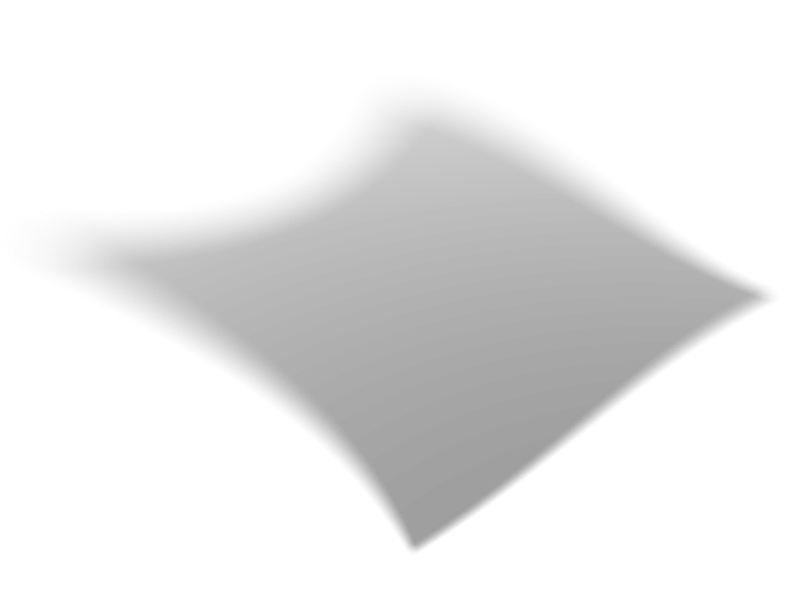
\includegraphics[width=\parampatchimagewidth]{figures/parametric_patch_shadow}};}
	\node at (0,0) {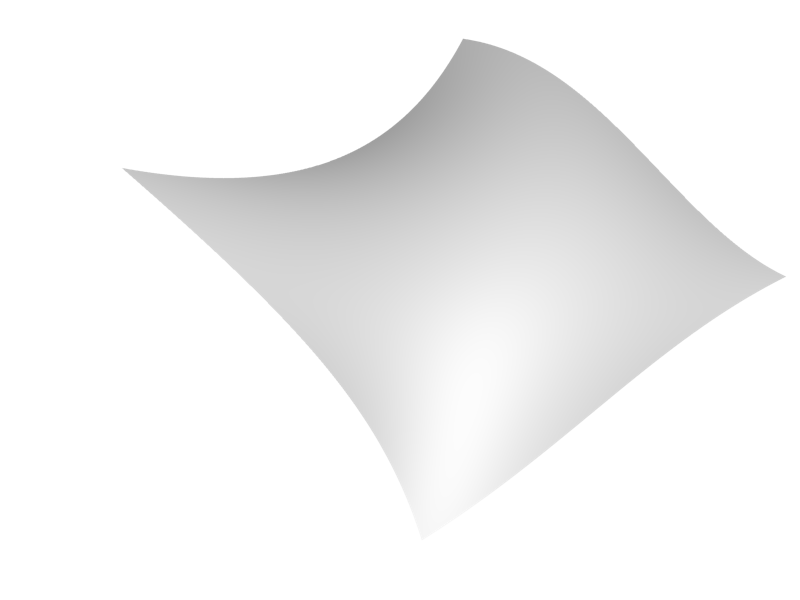
\includegraphics[width=\parampatchimagewidth]{figures/parametric_patch_surface}};
	\node at (0,0) {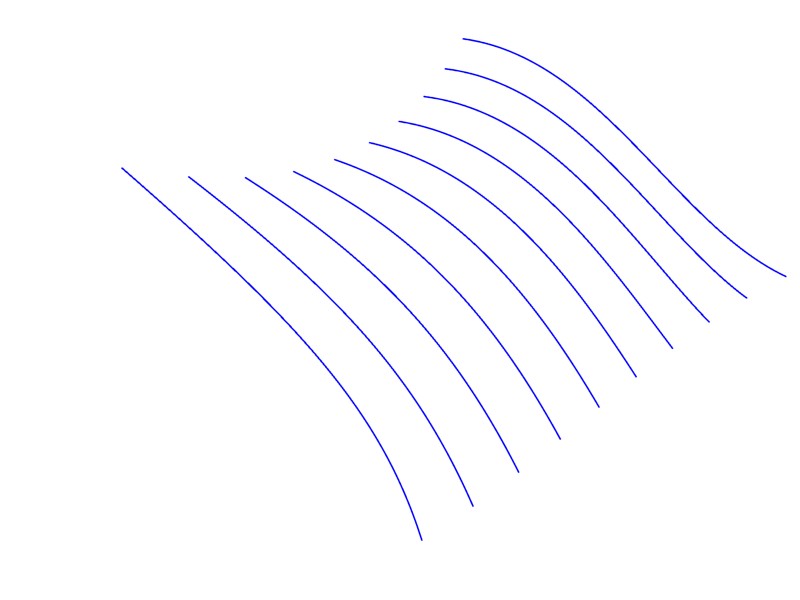
\includegraphics[width=\parampatchimagewidth]{figures/parametric_patch_isou}};
	\node at (0,0) {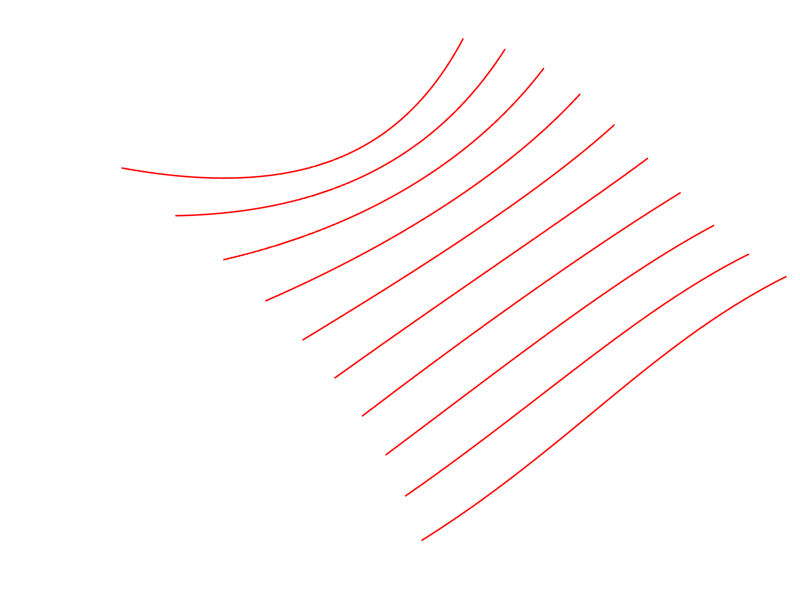
\includegraphics[width=\parampatchimagewidth]{figures/parametric_patch_isov}};
\end{tikzpicture}
\caption{Patch de surface paramétrique.}
\end{figure}


\section{Contributions}% aka "Description de la thèse/démarche"


\section{Organisation du manuscrit}